\documentclass[11pt]{article}

\usepackage[margin=1in]{geometry}
\usepackage{amsmath,amssymb,graphicx,enumerate}
\usepackage{caption}

\setlength{\parindent}{0pt}
\setlength{\parskip}{6pt}

\begin{document}

\title{Group Project 1: Statistical Analysis of a Currency (Japan)}
\author{Logan Rechin, Joe White\\ECO 442}
\date{}
\maketitle

\section*{Part 1: FRED Graph}

The following figure shows the daily nominal exchange rate for Japan against the U.S. dollar over the past 10 years. Denoted as:
\[
E_{\text{yen}/\$}
\]

\begin{figure}[h!]
\centering
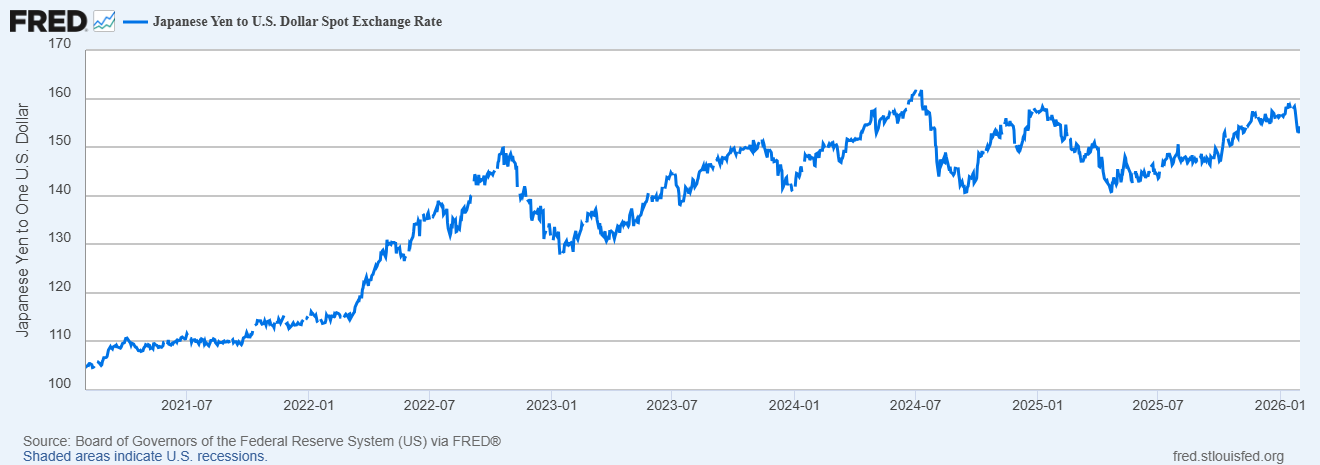
\includegraphics[width=0.95\textwidth]{fredgraph.png}
\caption{Japanese Yen per U.S. Dollar, daily nominal exchange rate.}
\end{figure}

\section*{Part 2: Hotel}

Japan's capital city is Tokyo. The hotel we chose is the Trunk Cat Street. The cost for one night is:
\[
P_{\text{yen}} = \text{\textyen}669{,}944.
\]

\section*{Part 3: Hotel Price}

To convert from yen into dollars:
\[
P_{\$}=\frac{P_{\text{yen}}}{E_{\text{yen}/\$}}.
\]

\begin{enumerate}[(1)]
\item \textbf{Wed Nov 26:} \quad $E_{\text{yen}/\$} = 156.38$
\[
P_{\$}^{\text{Nov 26}}
= \frac{669{,}944}{156.38}
= 4284.08,
\qquad \Rightarrow \qquad
P_{\$}^{\text{Nov 26}} \approx \$4{,}284.08
\]

\item \textbf{Fri Nov 28:} \quad $E_{\text{yen}/\$} = 156.17$
\[
P_{\$}^{\text{Nov 28}}
= \frac{669{,}944}{156.17}
= 4289.84,
\qquad \Rightarrow \qquad
P_{\$}^{\text{Nov 28}} \approx \$4{,}289.84
\]
\end{enumerate}

\section*{Part 4: Appreciation/depreciation}

The exchange rate fell from $156.38$ to $156.17$ yen per dollar. Since $E_{\text{yen}/\$}$ is yen per \$1, a decrease in $E_{\text{yen}/\$}$ means the yen appreciated.

Holding the hotel price fixed at \textyen669{,}944, the U.S. dollar price increased from approximately \$4{,}284.08 to \$4{,}289.84. The change in the dollar price was:
\[
\$4{,}289.84 - \$4{,}284.08 = \$5.76.
\]
The yen's appreciation made the hotel \$5.76 more expensive for a U.S. tourist on Nov 28 compared to Nov 26.

\end{document}
